%% LyX 2.0.2 created this file.  For more info, see http://www.lyx.org/.
%% Do not edit unless you really know what you are doing.
\documentclass[english]{beamer}
\usepackage[T1]{fontenc}
\usepackage[latin9]{inputenc}
\setlength{\parskip}{\bigskipamount}
\setlength{\parindent}{0pt}
\usepackage{color}
\usepackage{amsmath}
\usepackage{amssymb}
\usepackage{graphicx}

\makeatletter
%%%%%%%%%%%%%%%%%%%%%%%%%%%%%% Textclass specific LaTeX commands.
 % this default might be overridden by plain title style
 \newcommand\makebeamertitle{\frame{\maketitle}}%
 \AtBeginDocument{
   \let\origtableofcontents=\tableofcontents
   \def\tableofcontents{\@ifnextchar[{\origtableofcontents}{\gobbletableofcontents}}
   \def\gobbletableofcontents#1{\origtableofcontents}
 }
 \long\def\lyxframe#1{\@lyxframe#1\@lyxframestop}%
 \def\@lyxframe{\@ifnextchar<{\@@lyxframe}{\@@lyxframe<*>}}%
 \def\@@lyxframe<#1>{\@ifnextchar[{\@@@lyxframe<#1>}{\@@@lyxframe<#1>[]}}
 \def\@@@lyxframe<#1>[{\@ifnextchar<{\@@@@@lyxframe<#1>[}{\@@@@lyxframe<#1>[<*>][}}
 \def\@@@@@lyxframe<#1>[#2]{\@ifnextchar[{\@@@@lyxframe<#1>[#2]}{\@@@@lyxframe<#1>[#2][]}}
 \long\def\@@@@lyxframe<#1>[#2][#3]#4\@lyxframestop#5\lyxframeend{%
   \frame<#1>[#2][#3]{\frametitle{#4}#5}}
 \def\lyxframeend{} % In case there is a superfluous frame end
 \newenvironment{topcolumns}{\begin{columns}[t]}{\end{columns}}

%%%%%%%%%%%%%%%%%%%%%%%%%%%%%% User specified LaTeX commands.
\usepackage{tikz} 
\usepackage{pgfplots}
\usepackage{beamerthemebeamer}
\usepackage{movie15}

\AtBeginDocument{
  \def\labelitemi{\(\star\)}
  \def\labelitemii{ }
  \def\labelitemiii{ }
  \def\labelitemiv{ }
}

\makeatother

\usepackage{babel}
\begin{document}





\title[Short Paper Title]{Dynamics of quasi-particle states in a finite one-dimensional Bose
gas}


\author{Geert Kapteijns}


\institute{ITFA Bachelor's thesis}

\makebeamertitle


%\pgfdeclareimage[height=0.5cm]{institution-logo}{institution-logo-filename}

%\logo{\pgfuseimage{institution-logo}}



 \AtBeginSubsection[]{

  \frame<beamer>{ 

    \frametitle{Outline}   

    \tableofcontents[currentsection,currentsubsection] 

  }

}



%\beamerdefaultoverlayspecification{<+->}


\lyxframeend{}\lyxframe{Outline}

\tableofcontents{}




\lyxframeend{}\section{Introduction}


\lyxframeend{}\subsection[Basic Problem]{Motivations}


\lyxframeend{}\lyxframe{Motivations}

\textbf{J. Sato, E. Kaminishi, and T. Deguchi, Exact quantum dynamics
of yrast states in the finite 1D Bose gas, arXiv:1401.4262 {[}cond-mat.quant-gas{]}}


\pause{}

\textquotedbl{}Japanese guys\textquotedbl{} demonstrate dynamics of
a quasi-particle state in 1D Bose gas


\lyxframeend{}\lyxframe{Decay of quasi-particle}

\begin{figure}
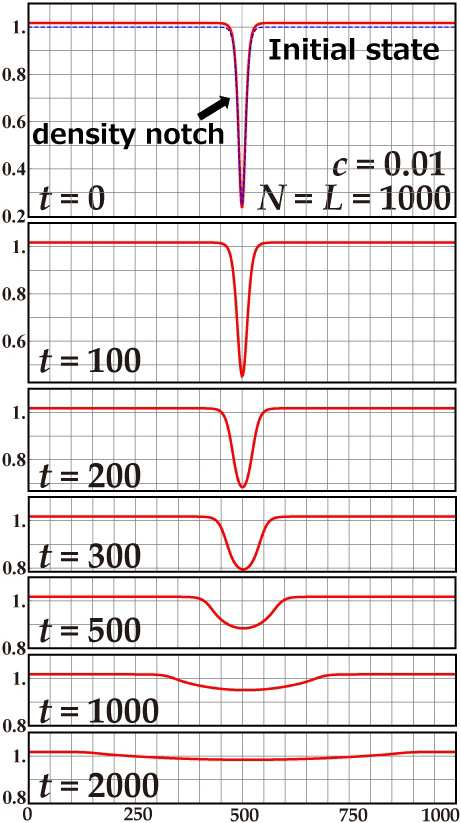
\includegraphics[scale=0.26]{density_profile_japanese}
\end{figure}



\lyxframeend{}\lyxframe{Aim}

Take a closer look at decay. Can we find an expression for it?


\lyxframeend{}


\lyxframeend{}\subsection{The Lieb-Liniger model}


\lyxframeend{}\lyxframe{The Lieb-Liniger model}

$N$ bosons on a ring with contact interaction (a delta peak.)


\pause{}

\begin{figure}
\noindent \centering{}\begin{tikzpicture}
	\definecolor{myblue}{RGB}{00,116,217}
	\draw (2,2) ellipse (4cm and 1cm);
	\draw[myblue, line width=7pt, line cap=round, dash pattern=on 0pt off 7\pgflinewidth] (2,2) ellipse (4cm and 1cm);
\end{tikzpicture}
\end{figure}



\pause{}

\[
H=-\sum_{i=1}^{N}\frac{\partial^{2}}{\partial x_{i}^{2}}+2c\sum_{i<j}\delta(x_{i}-x_{j})
\]



\lyxframeend{}\lyxframe{Bethe Ansatz}

Solvable through Bethe Ansatz: assume product of plane waves.


\pause{}

Leads to Bethe equations for bosons' pseudo-momenta:

\[
k_{j}L=2\pi I_{j}-2\sum_{l=1}^{N}\arctan(\frac{k_{j}-k_{l}}{c})\qquad j=1,\dots,N
\]



\pause{}

We label eigenstates by integers $I_{j}$.


\lyxframeend{}\lyxframe{Ground State}

\begin{figure}


\noindent \centering{}\begin{tikzpicture}
	\draw[dashed] (0,-0.5) -- (0,0.5);

	\foreach \x in {-2,...,2} {
		\filldraw (\x,0) circle (0.1cm);
	}
\end{tikzpicture}
\end{figure}



\pause{}

Ground state for $N=5$ labeled by:

\[
\{I_{j}\}=\{-2,-1,0,1,2\}
\]



\lyxframeend{}\lyxframe{Momentum}

Momentum given by:

\[
P=\frac{2\pi}{L}\sum_{j=1}^{N}I_{j}
\]



\pause{}

Groundstate: $I_{j}$'s sum to zero:

\[
P=0
\]



\lyxframeend{}\subsection{Excitations of the ground state}


\lyxframeend{}\lyxframe{Excitations of the ground state}

One-hole excitations: create a hole somewhere.

\begin{figure}
\begin{tikzpicture}
	\draw[dashed] (0,-0.5) -- (0,0.5);

	\foreach \x in {-2,...,1} {
		\filldraw (\x,0) circle (0.1cm);
	}

	\draw (2,0) circle (0.1cm);
	\filldraw (3,0) circle (0.1cm);

\end{tikzpicture}
\end{figure}



\pause{}

Labeled by:

\[
\{I_{j}\}=\{-2,-1,0,1,3\}
\]



\pause{}

For hole position $m$ (here $m=1$):
\begin{quotation}%{}
\texttt{
\[
P=\frac{2\pi}{L}m
\]
}
\end{quotation}%{}

\lyxframeend{}\subsection{Quasi-particle state}


\lyxframeend{}\lyxframe{Quasi-particle state}

Sum all one-hole excitations (\textbf{momentum eigenstates}) to get
a state that is localized in \textbf{position}.

\[
|\Psi\rangle=\frac{1}{\sqrt{N}}\sum_{m=-N}^{N}|P\rangle
\]



\pause{}

$|P\rangle$ represents the one-hole excitation with momentum $\frac{2\pi}{L}m$.


\lyxframeend{}\lyxframe{}

\begin{figure}


\begin{tikzpicture}
	\filldraw (-2,0) circle (0.1cm);
	\filldraw (-1,0) circle (0.1cm);
	\filldraw (-0,0) circle (0.1cm);
	\draw (1,0) circle (0.1cm);

	\filldraw (-2,-1) circle (0.1cm);
	\filldraw (-1,-1) circle (0.1cm);
	\draw (0,-1) circle (0.1cm);
	\filldraw (1,-1) circle (0.1cm);

	\filldraw (-2,-2) circle (0.1cm);
	\draw (-1,-2) circle (0.1cm);
	\filldraw (0,-2) circle (0.1cm);
	\filldraw (1,-2) circle (0.1cm);

	\filldraw (-1,-3) circle (0.1cm);
	\filldraw (0,-3) circle (0.1cm);
	\filldraw (1,-3) circle (0.1cm);

	\filldraw (-1,-4) circle (0.1cm);
	\filldraw (0,-4) circle (0.1cm);
	\draw (1,-4) circle (0.1cm);
	\filldraw (2,-4) circle (0.1cm);

	\filldraw (-1,-5) circle (0.1cm);
	\draw (0,-5) circle (0.1cm);
	\filldraw (1,-5) circle (0.1cm);
	\filldraw (2,-5) circle (0.1cm);

	\draw (-1,-6) circle (0.1cm);
	\filldraw (0,-6) circle (0.1cm);
	\filldraw (1,-6) circle (0.1cm);
	\filldraw (2,-6) circle (0.1cm);

	\draw[dashed] (0,-3.5) -- (0,-2.5);

\end{tikzpicture}

\end{figure}



\pause{}

All one-hole excitations for $N=3$.


\lyxframeend{}\section{Results}


\lyxframeend{}\subsection{Density profile: collapse of quasi-particle}


\lyxframeend{}\lyxframe{Density Profile}

\begin{figure}


\includemovie{1cm}{1cm}{density_typeII_symmetric_c1N100_animation_t_0-3.gif}

\end{figure}



\lyxframeend{}\lyxframe{Make Titles Informative. }
\begin{topcolumns}%{}


\column{5cm}
\begin{theorem}%{}
<1->In left column.
\end{theorem}%{}

\column{5cm}
\begin{corollary}%{}
<2->In right column.\\
New line
\end{corollary}%{}
\end{topcolumns}%{}

\lyxframeend{}\subsection{$t^{-1}$ decay behaviour and lifetime parameter $\tau$}


\lyxframeend{}\section*{Summary}


\lyxframeend{}\lyxframe{Summary}
\begin{itemize}
\item The \textcolor{red}{first main message} of your talk in one or two
lines.
\item The \textcolor{red}{second main message} of your talk in one or two
lines.
\item Perhaps a \textcolor{red}{third message}, but not more than that.
\end{itemize}


\vskip0pt plus.5fill
\begin{itemize}
\item Outlook

\begin{itemize}
\item What we have not done yet.
\item Even more stuff.
\end{itemize}
\end{itemize}

\lyxframeend{}

\appendix

\lyxframeend{}\section*{Appendix}


\lyxframeend{}\subsection*{For Further Reading}


\lyxframeend{}\lyxframe{[allowframebreaks]For Further Reading}

\beamertemplatebookbibitems
\begin{thebibliography}{References}
\bibitem{Author1990}A. Author. \newblock\emph{Handbook of Everything}.\newblock
Some Press, 1990.\beamertemplatearticlebibitems

\bibitem{Someone2002}S. Someone.\newblock On this and that\emph{.}
\newblock\emph{Journal on This and That}. 2(1):50--100, 2000.

\end{thebibliography}

\lyxframeend{}
\end{document}
